\documentclass[12pt]{amsart}
\usepackage{amssymb}
\usepackage{cite}
\usepackage{array}
\usepackage{booktabs}
\usepackage{mdwtab}
\usepackage{mathtools}
\usepackage{lmodern}
\usepackage{microtype}
\usepackage[T1]{fontenc}
\usepackage[utf8]{inputenc}
\usepackage{hyphenat}
\usepackage{enumitem}
\usepackage{mathabx}
\usepackage{color}
\usepackage[pdftex]{graphicx}
\usepackage[pdftex,margin=1in,lmargin=0.75in,rmargin=1.5in,marginparwidth=1.2in]{geometry}
\usepackage[bookmarks=true, bookmarksopen=true,%
    bookmarksdepth=3,bookmarksopenlevel=2,%
    colorlinks=true,%
    linkcolor=blue,%
    citecolor=blue,%
    filecolor=blue,%
    menucolor=blue,%
    urlcolor=blue]{hyperref}
\hypersetup{pdftitle={Metric Geometry: Class Notes}}
\hypersetup{pdfauthor={Dylan P. Thurston et al.}}
\usepackage{url}
\usepackage{tikz}
\usetikzlibrary{arrows}
\tikzstyle{every picture}=[> = to]
% Style for labels on arrows in commutative diagrams
\tikzset{cdlabel/.style={execute at begin node=$\scriptstyle,execute at end node=$}}
\tikzset{implication/.style={double equal sign distance, -implies}}
\tikzset{biimplication/.style={double equal sign distance, implies-implies}}

% A binary operator with a subscript on both sides (and correct spacing)
% Name stands for subscript-operator-subscript
% Perhaps this should be using \manyindices?
\newcommand{\sos}[3]{\mathbin{{}_{#1}\mathord#2_{#3}}}

% manyindices
% Adapted from code by "bza" in comp.text.tex, Feb. 7, 2006
%% USAGE:
%%
%% \manyindices#1#2#3#4#5
%%
%% #1=lower left index
%% #2=upper left index
%% #3=lower right index
%% #4=upper right index
%% #5=main symbol
\makeatletter
\newcommand\mi@kern[1]{%
  \settowidth\@tempdima{$\mi@obj^{#1}$}
  \kern-\@tempdima
  #1
  \settowidth\@tempdima{$\mi@obj$}
  \kern\@tempdima
}

\newtoks\mi@toksp
\newtoks\mi@toksb
\DeclareRobustCommand{\manyindices}[5]{
  \def\mi@obj{#5}
  \mi@toksp\expandafter{\mi@kern{#2}}
  \mi@toksb\expandafter{\mi@kern{#1}}
  \@mathmeasure4\textstyle{#5_{#1}^{#2}}
  \@mathmeasure6\textstyle{#5_{#3}^{#4}}
  \dimen0-\wd6 \advance\dimen0\wd4
  \@mathmeasure8\textstyle{\hphantom{{}_{#1}^{#2}}#5^{\the\mi@toksp#4}_{\the\mi@toksb#3}}
  \hbox to \dimen0{}{\kern-\dimen0\box8}
}
\makeatother 

% Left sub/super scripts
% \lsup is a temporary definition until something better is worked out
% Use \lsupv if the next argument is vertical
\newcommand{\lsub}[2]{{}_{#1}#2}
\newcommand{\lsup}[2]{{}^{#1}\mskip-.6\thinmuskip#2}
\newcommand{\lsupv}[2]{{}^{#1}#2}
\newcommand{\lsubsup}[3]{\manyindices{#1}{\mskip.6\thinmuskip#2\mskip-.6\thinmuskip}{}{}{\mathord{#3}}}
\newcommand{\lsubsupv}[3]{\manyindices{#1}{\mskip.2\thinmuskip#2\mskip-.2\thinmuskip}{}{}{\mathord{#3}}}

\newcounter{saveenum}

% Read the file, if it exists
\newread\testin
\def\maybeinput#1{
\openin\testin=#1
\ifeof\testin\typeout{Warning: input #1 not found}\else\input#1\fi
\closein\testin
}

\def\mathcenter#1{%
  \vcenter{\hbox{$#1$}}%
}

\def\graph#1{
        \includegraphics{#1}
}

\def\mathgraph#1{
        \mathcenter{\graph{#1}}
}

\def\mfig#1{
        \mathcenter{\includegraphics{#1}}
}

\def\mfigb#1{
        \mathcenter{\includegraphics[trim=-1 -1 -1 -1]{#1}}
}

\newcommand{\DPTtodo}[1]{\todo[color=green!40]{#1}}

\newcommand{\arXiv}[1]{\href{http://arxiv.org/abs/#1}{arXiv:#1}}


% \colon with an optional line break. From https://groups.google.com/forum/#!topic/comp.text.tex/Ts7R4WDTK-M
\renewcommand{\colon}{\nobreak\mskip2mu\mathpunct{}\nonscript
  \mkern-\thinmuskip{:}\allowbreak\mskip6muplus1mu\relax}

%%% Local Variables: 
%%% mode: latex
%%% TeX-master: "main"
%%% End: 

% General use
\newcommand{\RR}{\mathbb R}
\newcommand{\CC}{\mathbb C}
\newcommand{\ZZ}{\mathbb Z}
\newcommand{\QQ}{\mathbb Q}
\newcommand{\PP}{\mathbb P}
\newcommand{\EE}{\mathbb E}
\newcommand{\HH}{\mathbb H}
\newcommand{\NN}{\mathbb N}

\newcommand{\comma}{\mathbin ,}
\newcommand{\conn}{\mathbin \#}
\newcommand{\sltwo}{{{\mathfrak{sl}}_2}}
\renewcommand{\sl}{\mathfrak{sl}}
\newcommand{\gl}{\mathfrak{gl}}
\newcommand{\fg}{{\mathfrak g}}
\newcommand{\eps}{\varepsilon}
\newcommand{\abs}[1]{{\lvert #1 \rvert}}
\newcommand{\norm}[1]{{\lVert #1 \rVert}}
\newcommand{\OneHalf}{{\textstyle\frac{1}{2}}}

% Synonyms for commands I never remember
\newcommand{\isom}{\cong}
\newcommand{\superset}{\supset}
\newcommand{\bigcircle}{\bigcirc}
\newcommand{\contains}{\ni}
\newcommand{\tensor}{\otimes}
\newcommand{\bdy}{\partial}

% Stupid overloading.
\newcommand{\lbracket}{[}
\newcommand{\rbracket}{]}

% More delimiters
\DeclarePairedDelimiter\ceil{\lceil}{\rceil}
\DeclarePairedDelimiter\floor{\lfloor}{\rfloor}

% Various operators.
\DeclareMathOperator{\ad}{ad}
\DeclareMathOperator{\Ad}{Ad}
\DeclareMathOperator{\End}{End}
\DeclareMathOperator{\sign}{sign}
\DeclareMathOperator{\Sym}{Sym}
\DeclareMathOperator{\tr}{tr}
\DeclareMathOperator{\Hom}{Hom}
\DeclareMathOperator{\vol}{vol}
\DeclareMathOperator{\rank}{rank}
\DeclareMathOperator{\im}{im}
\DeclareMathOperator{\Gr}{Gr}

% Linear groups
\DeclareMathOperator{\ISO}{\mathit{ISO}}
\DeclareMathOperator{\SO}{\mathit{SO}}
\DeclareMathOperator{\GL}{\mathit{GL}}
\DeclareMathOperator{\SL}{\mathit{SL}}
\DeclareMathOperator{\PSL}{\mathit{PSL}}

% Special knots
\newcommand{\unknot}{\bigcircle}

% Theorems
\theoremstyle{plain}
\newtheorem{theorem}{Theorem}
\newtheorem{proposition}{Proposition}
\newtheorem{lemma}[proposition]{Lemma}
\newtheorem{corollary}[proposition]{Corollary}
\newtheorem{claim}[proposition]{Claim}
\newtheorem{conjecture}[proposition]{Conjecture}
\newtheorem{observation}[proposition]{Observation}

\theoremstyle{definition}
\newtheorem{definition}[proposition]{Definition}
\newtheorem{exercise}[proposition]{Exercise}
\newtheorem{question}[proposition]{Question}
\newtheorem{problem}[proposition]{Problem}

\theoremstyle{remark}
\newtheorem{example}[proposition]{Example}
%\newtheorem{hint}[proposition]{Hint}
\newtheorem*{remark}{Remark}
%\newtheorem{apology}[proposition]{Apology}
%\newtheorem{warning}[proposition]{Warning}

% Hyphenation.
\hyphenation{Thurs-ton}

% Noting scribes
\newcommand{\scribe}[2]{\marginpar{\small #1\\\texttt{#2}}}

%%% Local Variables: 
%%% mode: latex
%%% TeX-master: "main"
%%% TeX-master: t
%%% End: 


\graphicspath{{draws/}{}}

\begin{document}
\title[Metric Geometry: Class Notes]{Metric Geometry: Class Notes\\
  \small Fall 2018}

\author[Thurston]{Dylan~P.~Thurston}
\author{members of M531}
\date{\today}

\maketitle

\tableofcontents

\section{Metric spaces}
\label{sec:metric-spaces}

\scribe{Dylan Thurston}{2018-08-20}
\begin{definition}
  A \emph{metric space} is a set~$X$ together with a \emph{distance
    function} $d \colon X \times X \to \RR_{\ge 0} \cup \{\infty\}$
  satisfying the following axioms for all $x,y,z \in X$.
  \begin{itemize}
  \item \textbf{(Reflexive)} $d(x,x) = 0$.
  \item \textbf{(Triangle inequality)} $d(x,z) \le d(x,y) + d(y,z)$.
    (Going straight from $x$ to~$z$ is at least as good as going from
    $x$ to~$y$ and then from $y$ to~$z$.)
  \item \textbf{(Symmetry)} $d(x,y) = d(y,x)$.
  \item \textbf{(Distinguishable)} If $d(x,y) = 0$, then $x = y$.
  \end{itemize}
\end{definition}

\begin{example}
  $\RR^2$, with its standard Euclidean metric $d_{\text{Eucl}}$, is a
  metric space.
\end{example}

\begin{example}
  $\ZZ^2$, with the metric $d_{\text{Eucl}}$ induced as a subset of
  $\RR^2$, is a metric space.
\end{example}

\begin{example}
  $\RR^2$ with the taxicab metric defined by
  \[
    d_{\text{taxi}}\bigl((x_1,x_2),(y_1,y_2)\bigr) = \abs{x_1 - y_1} +
    \abs{x_2 - y_2},
  \]
  is a metric space. In this space, the balls are diamond-shape rather
  than circles.
\end{example}

\begin{example}
  The standard unit sphere $S^2 \subset \RR^3$ with the extrinsic
  metric $d_{\text{extr}}$ induced
  as a subset of $\RR^3$ is a metric space.
\end{example}

If you drop the condition that the metric be distinguishable, you get
a \emph{pseudometric} space. For instance, $\RR^2$ with the metric
that is identically $0$ is a pseudometric space, as is $\RR^2$ with
the metric that only measures distance along the first coordinate.

If you drop the condition that the metric is symmetric, you get an
\emph{asymmetric metric}. These are less standard, despite occurring in
natural situations.

\begin{example}
  An (undirected) graph gives a metric space, where the points are the
  vertices and the distance between two vertices is the minimum number
  of edges you need to cross to get from one vertex to another. A
  \emph{directed} graph gives an asymmetric metric space, where you
  are only allowed to cross edges in the direction of the arrow.
\end{example}

Another real-world example of an asymmetric metric is travel
difficulty; it is much harder to walk from the bottom of a mountain to
the top than the other way around.

A metric naturally gives you a \emph{topology}, for instance defining
continuous maps.
\begin{definition}
  If $X$ and $Y$ are metric spaces, a function $f \colon X \to Y$ is
  \emph{continuous} if
  \[
  \forall x \in X, \,\forall \epsilon > 0,\,
  \exists \delta > 0,\,\forall y \in X\colon
  d_X(x,y) < \delta \Rightarrow d_Y(f(x),f(y)) < \epsilon
  \]
  or, loosely, if points sufficiently close to each other in~$X$ are
  close in~$Y$. Subtle variations yield different concepts; for
  instance, if you move the clause ``$\forall y \in X$'' to the
  beginning, then you get the notion of \emph{uniform continuity},
  which depends on the metric and not just on the topology.
\end{definition}

\section{Quasi-isometries (preview)}
\label{sec:quasi-isom-1}
A metric gives a lot more structure than just a topology. On the other
end of the spectrum of what a metric gives you, we have the notion of
\emph{quasi-isometric embedding}, which ignores what happens on the
small scale (which is the only thing relevant to the topology), and in
stead focuses on the behavior on grand scales.

\begin{definition}
  If $X$ and $Y$ are metric spaces, a function $f \colon X \to Y$ is a
  \emph{quasi-isometric embedding} if there are constants $K >1$ and
  $C > 0$ so that $\forall x,y \in X$,
  \[
    \frac{d_X(x,y) - C}{K}
      \le d_Y(f(x), f(y)) \le
        K d_X(x,y) + C.
  \]
  That is, distances in $X$ are distorted by $f$ by at most a
  multiplicative factor~$K$ and an additive constant~$C$.
\end{definition}

\begin{example}
  The identity map
  $(\RR^2, d_{\text{Eucl}}) \to (\RR^2, d_{\text{taxi}})$ is a
  quasi-isometry with $K = \sqrt{2}$ and $C=0$, as is the identity map
  going the other way.
\end{example}

\begin{example}
  The inclusion map
  $(\ZZ^2,d_{\text{Eucl}}) \hookrightarrow (\RR^2,d_{\text{Eucl}})$ is a
  quasi-isometry with $K=1$ and $C=0$, i.e., an \emph{isometry}.
\end{example}

\begin{example}
  The map $f \colon (\RR^2, d_{\text{Eucl}}) \to (\ZZ^2,
  d_{\text{Eucl}})$ defined by
  \[
    f\bigl((x_1,x_2)\bigr) = (\ceil{x_1}, \ceil{x_2})
  \]
  is a quasi-isometry with $K=1$ and $C=2$. (Can this value of $C$ be
  improved?) Note that $f$ is not continuous.
\end{example}

\begin{example}
  There is a quasi-isometry from $(S^2, d_{\text{extr}})$ to
  $(\RR^2, d_{\text{Eucl}})$; for instance, project on to the plane, or
  more simply map all of $S^2$ to a single point. However, there is no
  quasi-isometry in the other direction.
\end{example}

\begin{exercise}
  Verify the above assertions.
\end{exercise}

\begin{definition}
  A quasi-isometric embedding $f \colon X \to Y$ is a
  \emph{quasi-isometry} if every point in~$Y$ is near the image
  of~$X$, or, precisely, if there is a constant $C_2 > 0$ so that
  \[
    \forall y \in Y,\, \exists x \in X\colon d_Y(f(x),y) < C_2.
  \]
\end{definition}

\begin{exercise}
  Show that if $f \colon X \to Y$ is a quasi-isometry, then there is
  also a quasi-isometry $g \colon Y \to X$. What can you
  say about the composition $g \circ f$?
\end{exercise}

\begin{exercise}
  Show that a metric space $(X,d)$ is quasi-isometric to a point iff
  $d$ is bounded.
\end{exercise}

\begin{exercise}
  If $X$ is any metric space, show that any map $f \colon X \to X$
  that moves each point a (globally) bounded amount is a
  quasi-isometry. (For instance, $f$ need not be continuous.)
\end{exercise}

The notion of quasi-isometry is quite useful in group theory, since it
can give us some notion of large-scale geometry even on discrete sets
like a fundamental group. For instance, the following theorem is true.

\begin{theorem}
  If $X$ is a compact manifold,
  then its fundamental group $\pi_1(X)$ is quasi-isometric to its
  universal cover $\wt X$.
\end{theorem}

Here, we use the metric on $\pi_1(X)$ coming from its \emph{Cayley
  graph}, which we will come back to later.

\begin{example}
  For $X = S^1$, we have seen that $\pi_1(S^1) = \ZZ$ is
  quasi-isometric to $\widetilde{S^1} = \RR$. For $X = S^2$, we have
  seen that $\pi_1(S^2) = \{e\}$ is quasi-isometric to
  $\widetilde{S^2} = S^2$.
\end{example}

\begin{question}
  Is there an unbounded metric $d$ on $\RR^2$, inducing the standard
  topology, so that $(\RR^2,d)$ is not quasi-isometric to
  $(\RR^2,d_{\text{Eucl}})$?
\end{question}

\begin{question}
  What properties of metric spaces are preserved by quasi-isometries?
\end{question}

We will consider quasi-isometry and other ``quasi'' notion more later
in the course. In the meantime, you can think about the questions
above as we go along.

\section{Lengths of curves}
\label{sec:lengths}

\begin{definition}
  A \emph{curve}~$\gamma$ in a metric space $(X,d)$ is a continuous map
  \[
    \gamma\colon [0,1] \to X,
  \]
  using the standard metric on the interval.
\end{definition}

What should the length of a curve be? For sufficiently nice curves in
$(\RR^2, d_{\text{Eucl}})$, we can use the calculus definition and set
the length to be
\begin{equation}
  \label{eq:length-eucl}
  \int_0^1 \abs{\gamma'(t)}\,dt.
\end{equation}
However, this doesn't work if the target space has no notion of
differentiation. It doesn't even always work well in $\RR^2$.

\begin{example}
  Take $\gamma$ to be a nice curve in $\RR^2$ (say a semi-circle), and
  let $\phi \colon [0,1] \to [0,1]$ be a weakly monotonic
  reparametrization function (with $\phi(0) = 0$ and $\phi(1) = 1$),
  so that its derivative is almost everywhere~$1/2$ (like the
  \href{https://en.wikipedia.org/wiki/Cantor_function}{Devil's
    Staircase}, with an additional linear function added). Then we
  expect $\gamma \circ \phi$ to describe the same geometric curve as
  $\gamma$ and have the same length. But the
  integral~(\ref{eq:length-eucl}) (to the extent it exists) gives a
  different answer.%
  \footnote{In class, I suggested taking $\phi$ to be a monotonic,
    nowhere-differentiable function, but no such functions exist.}
\end{example}

To get something more general, we look at subdivisions.

\begin{definition}\label{def:length}
  If $\gamma$ is a curve in a metric space~$X$, its \emph{length} is
  defined to be
  \begin{equation}\label{eq:length}
    \ell(\gamma) = \sup \sum_{i=0}^k d(\gamma(t_i), \gamma(t_{i+1})),
  \end{equation}
  where the supremum runs over all subdivisions of $[0,1]$ into
  a finite number of subintervals at
  \[
    0 = t_0 < t_1 < \cdots < t_k < t_{k+1} = 1.
  \]
\end{definition}

Note that if we make a subdivision finer by adding an extra point, the
supremand in~(\ref{eq:length}) can only increase (by the triangle
inequality). This helps with convergence.

\begin{exercise}
  If you know about the theory of
  \href{https://en.wikipedia.org/wiki/Net_(mathematics)}{nets}, verify
  that subdivisions of the interval form a directed set under refining
  subdivisions, and that supremum can be replaced by limit of a net
  in Equation~(\ref{eq:length}).
\end{exercise}

\scribe{Tom Yerger}{2018-08-22}

\begin{example}
There are plenty of examples of curves in metric spaces with infinite length. Consider the (ternary) Dragon curve, defined as follows:

At step 1 of the construction, we have  straight line path in $\mathbb{R}^2$ between two points. At each step of the construction, we bisect all segments of the curve, and bend the curve into equilateral triangles in opposite directions, as pictured below. Some trigonometry (as demonstrated in the image) shows that the length of the curve is bounded below by a geometric series with common ration $\frac{2}{\sqrt{3}}$, which is of course bigger than $1$.

One can check that the limit of this process is a continuous curve in the plane. Some steps of the construction are depicted below.
\begin{center}
  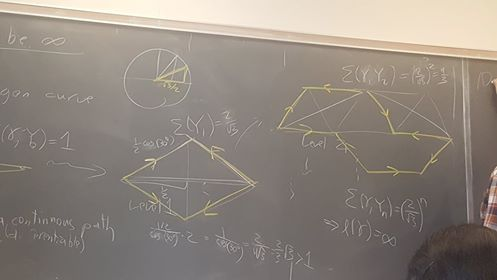
\includegraphics[width=4in]{2018-08-22-Dragon1}
\end{center}

\pagebreak[2]
Here is a better approximation of the limit.
\begin{center}
  
\includegraphics[width=3in]{2018-08-22-Dragon2}
\end{center}
\end{example}


The previous example motivates the following definition:

\begin{definition} A curve $\gamma$ will be called \textit{rectifiable} if $\ell (\gamma) < \infty$. Otherwise it is called \textit{non-rectifiable}.

\end{definition}

Some metric spaces are so wild that they do not have any non-constant rectifiable curves between points. One way this can happen is if the metric space is discrete, in the sense that all points are isolated (not necessarily carrying the discrete metric). There are of course no continuous paths connecting isolated points! Thus, any lattice in $\mathbb{R}^n$ with any metric at all gives an example. However, there are more interesting examples of non-discrete spaces.

\begin{example}
Let $X = (\mathbb{R}, \rho)$, where $\rho(x,y) = \sqrt{|x-y|}$. We claim that this space has no non-constant rectifiable paths. We will prove this in two steps. First, we will show that the path $\gamma: [a,b] \hookrightarrow \mathbb{R}$ is not rectifiable as a lemma. Then we will treat the general case.

For the lemma, consider the naive sequence of subdividing the interval into $n$ equal parts. If we do this, then all the distance terms are precisely $\sqrt{\frac{|b-a|}{n}}$, so the terms of this sequence as $n \to \infty$ are increasing like $\sqrt{n}$, which diverges.

Now for the heart of the proof, observe that if the curve is non-constant, it must pass through the midpoint $(b-a)/2$ at some $t$, by the intermediate value theorem. We take this to be our first partition. The $n$-th partition is constructed by choosing one $t_i$ for each time that the curve passes over $i(b-a)/n$. This partition's length will be bounded below in terms of the previous example, and so also diverges. Thus the lemma implies that all non-constant curves are non-rectifiable.
\end{example}

\begin{remark}
The same argument works analogously with any metric of the form $\rho(x,y) = |y-x|^\epsilon$, for $0 < \epsilon < 1$. One must check that this defines a metric, but after doing so, the same argument works analogously. Taking $\epsilon \to 1$, we get the usual metric. Taking $\epsilon \to 0$, the limiting metric is the discrete metric, which may give some intuition for why such curves are non-rectifiable, as there are no non-constant curves at all in a discrete space. One can think of $\epsilon < 1$ as "close" to the degenerate case of the discrete metric.
\end{remark}

There are a handful of useful properties of the length function that are worth recording, even if they are elementary:

\begin{enumerate}
    \item $\ell(\gamma) \geq d(\gamma(a), \gamma(b)$. 
    \item The length function is invariant under a monotonic reparameterization. 
    \item If $\gamma_1:[a,b] \to X$, and $\gamma_2:[b,c] \to X$, with $\gamma_1(b) = \gamma_2(b)$, then the amalgamated curve $\Gamma$ has $\ell(\Gamma) = \ell(\gamma_1) + \ell(\gamma_2)$
    \item $\ell(\gamma|_{[c,d]})$ is a continuous function of $c,d$
    \item $\ell(\gamma)$ is a lower semicontinuous functon in the topology of uniform convergence.
\end{enumerate}

\begin{proof}

Each of these results, with the exception of (5) is an immediate consequence of the definitions.  For this, let $\gamma_i$ be a sequence of curves converging uniformly to $\gamma$, as in the statement. Choose a partition $Y$ so that $\sum(\gamma, Y)$ approximates $\ell(\gamma)$. We have 

$$\sum(\gamma, Y) \leq \ell(\gamma) \leq \sum(\gamma, Y) + \epsilon $$

By uniform convergence, making $i$ large, we can arrange that $d(\gamma_i(t), \gamma(t)) < \delta$, for any $\delta > 0$. Now by choosing the same partition for $\gamma_i$, we may approximate the lengths of $\gamma$ in terms of $\gamma_i$, by travelling a distance at most $\delta$ from $\gamma$ to $\gamma_i$, and then travelling along $\gamma_i$, and then back to the tail of $\gamma$. This gives an upper bound for the length of $\gamma$ by writing 

$$\sum(\gamma, Y) + \epsilon \leq 2 \delta N + \sum(\gamma_i, Y) + \epsilon \leq \ell(\gamma_i) + 2 \delta N  + \epsilon$$

where $N$ is the number of points of the partition $Y$. Since $\epsilon$ and $\delta$ are arbitrary, this shows that $\ell(\gamma) \leq \liminf \ell(\gamma_i)$, which is equivalent to lower semicontinuity.

\end{proof}

Observe that the following image indicates that lower semicontinuity is all that can be asked for. The image displays a sequence of functions converging pointwise, but the lengths are constant and not converging to the length of the limit.

\begin{center}
  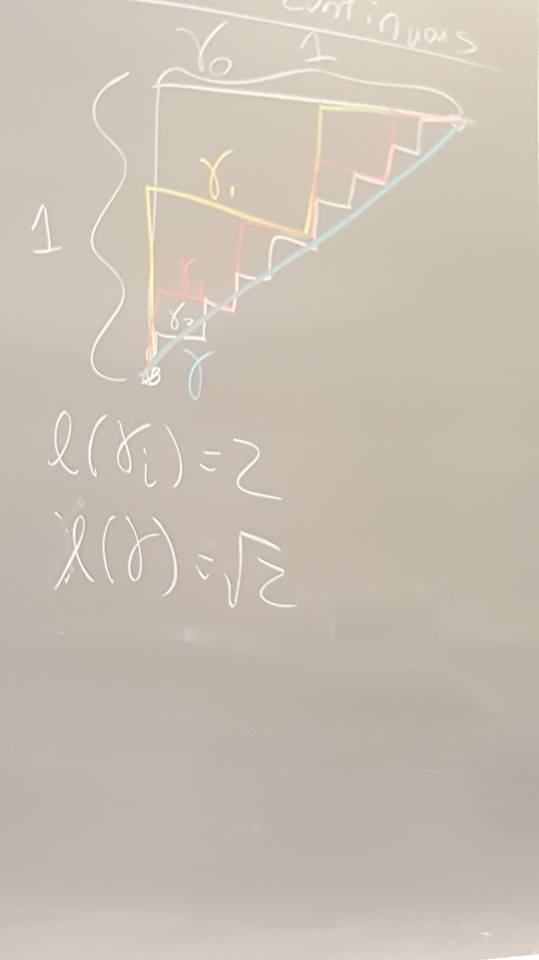
\includegraphics[width=3in]{2018-08-24}
\end{center}

Measuring distances along curves is such a natural idea that we give spaces where it is feasible a name:

\begin{definition}
The intrinsic metric on a metric space $X$ is defined by $\rho(x,y) = \inf_\gamma \ell(\gamma)$, where $\gamma$ is a curve $[a,b] \to X$ satisfying $\gamma(a) = x, \gamma(b) = y$.  If the intrinsic metric on a space is equal to the metric it came equipped with, we call $X$ a \textit{length space}. Note that unlike ordinary metric spaces, here we will define $\rho(x,y) = \infty$ if there is no rectifiable path between $x$ and $y$, meaning that our metric space takes values in $[ 0, \infty ]$
\end{definition}

In a non-length space, a wide variety of behaviors are possible. The differing metrics do not even need to induce the same topologies. Consider the following examples:

\begin{example}
Let $X_1$ be a spiral, given in polar coordinates by $r = t/(t+1)$ and $\theta = t$, together with the limiting boundary circle of radius $1$. The induced metric as a subspace of $\mathbb{R}^2$ is quite different, as points which are quite close together as points in $\mathbb{R}^2$ can be extremely far apart. Furthermore, observe that there is no path from a point on the spiral to the boundary circle, and yet in am arbitrary neighborhood of a boundary point in the Euclidean metric, we can find infinitely many points from the spiral.
\end{example}

\begin{example}
Consider $\mathbb{R}^2$ with the following 'comb' metric. Let $p = (x_1, y_1)$, $q = (x_2, y_2)$. Then $d(p,q)= |x_2 - x_1| + |y_2 - y_1|^\epsilon$, for $0 \leq \epsilon < 1$. By the previous discussion, no rectifiable path can move in the vertical direction. This is also clearly a metric, by that same discussion, as it is a sum of two metrics in each factor. However, in this topology, the plane is not even connected. It is a disjoint union of uncountably many horizontal straight lines. 
\end{example}

In spite of how badly the topology can change, the following proposition demonstrates that rectifiable curves are the 'correct' class of curves to be studying for metric geometry:

\begin{proposition}
Suppose $\gamma:[a,b] \to X$ is rectifiable in $d$. Then it is also rectifiable in the intrinsic metric $\hat{d}$ and $\ell_d (\gamma) = \ell_{\hat{d}} (\gamma)$.
\end{proposition}

\begin{proof}
The inequality $\ell_d (\gamma) \leq \ell_{\hat{d}} (\gamma)$ is completely trivial. For the reverse inequality, pick a aprtition $Y$ of the domain $[a,b]$, and consider $\sum(\gamma, Y)$. We have $\sum(\gamma, Y) = \sum \hat{d}(\gamma(t_i), \gamma(t_{i+1})) \leq \sum \ell_d(\gamma|_{[t_i, t_{i+1}]})$, since $\gamma$ is just one curve connecting these points, and $\hat{d}$ is defined to be the inf over all such curves. But additivity of $\ell$ above implies this is just $\ell_d (\gamma)$.
\end{proof}

As a corollary, this implies that the induced metric does not itself induce another new metric. In other words, $\hat{\hat{d}} = \hat{d}$. Also, note that we must have $\gamma$ rectifiable. If $\gamma$ is not assumed rectifiable, the comb metric above can furnish us with examples of curves which are not even continuous in the induced metric.

In many examples of familiar metric spaces, especially complete metric spaces, the infimum is attained. This motivates the following definition:

\begin{definition}
A \textit{geodesic} $\gamma:[a,b] \to X$ is a curve attaining the infinimum between $\gamma(a)$ and $\gamma(b)$. A \textit{geodesic space} is a space in which every pair of points has at least one geodesic. It need not be unique. 
\end{definition}

\begin{example}
The plane, sphere, and hyperbolic space are all geodesic spaces. Puncturing any of these spaces makes them no longer geodesic spaces, as seen by picking any two points for which the geodesic would have had to pass through that point, had it existed. In the Euclidean and hyperbolic space, geodesics are unique. However, on the sphere, they need not be. Choosing two antipodal means that any arc of a great circle forming half an equator will be a geodesic connecting these points.

As a warning, a geodesic in this sense is not the same as a Riemannian geodesic. In Riemannian geometry, the equator of a sphere is regarded as a geodesic. However, in our sense, it is not, as any curve going beyond the antipode on a sphere will not be the infimal length (as you are going 'the long way' around the sphere).
\end{example}

\begin{exercise}
Suppose that $\gamma$ is a rectifiable curve. Show that there is a reparametrization of $\gamma$, $\gamma'$ such that $\gamma = \gamma' \circ \varphi$, so that $\gamma'$ is now parametrized by arc length. That is to say, $\ell(\gamma'|_{[a,b]}) = b - a$ for any $[a,b]$ in the domain of $\gamma'$.
\end{exercise}
\scribe{Aric Wheeler}{8-27-2018}
\begin{exercise}
Suppose $\gamma:[a,b]\rightarrow X$ is a rectifiable curve, then:
\begin{enumerate}
    \item Define $\phi(t):=\ell(\gamma|_{[a,t]})$. Then $\phi$ is a continuous, weakly monotonic function.\\
    \item Fix $s\le\ell(\gamma)$, define a new curve $\bar{\gamma}(s):=\gamma(t)$ for some $t\in\phi^{-1}(\{s\})$. Then $\bar{\gamma}$ is well-defined and continuous.\\
    \item $\bar{\gamma}\circ\phi=\gamma$, $\bar{\gamma}$ is said to be \underline{parameterized by arc length}, i.e. $\ell(\bar{\gamma}|_{[s,t]})=|t-s|$.
\end{enumerate}
\end{exercise}

\section{Hopf-Rinow/Cohn-Vassen}
Today: We will show that every complete, locally compact length space is a geodesic space.\\
\begin{definition}
\begin{itemize}
    \item For $X$ a metric space, set $|a-b|=d(a,b)$.
    \item Let $X$ be a metric space, for a pair $a,b\in X$ a \underline{midpoint between a,b} is a point $c\in X$ such that $|a-c|=|b-c|=\frac{1}{2}|a-b|$.
    \item An \underline{$\epsilon$-midpoint} is a point $c\in X$ such that $|a-c|,|b-c|\le \frac{1+\epsilon}{2}|a-b|$.
\end{itemize}
\end{definition}

\begin{proposition}
\begin{itemize}
    \item In a geodesic space, every pair of points has a midpoint.\\
    \item In a length space, every pair of points has an $\epsilon$-midpoint for each $\epsilon>0$.
\end{itemize}
\end{proposition}

\begin{proof}
\begin{itemize}
    \item Given $a,b\in X$, let $\gamma:[0,|a-b|]\rightarrow X$ be a geodesic parameterized by arc-length. Then the point $c=\gamma(\frac{|a-b|}{2})$ is a midpoint.
    \item Take a $\gamma:[0,|b-a|]\rightarrow X$ a curve connecting $a,b$ parameterized by arc length such that $\ell(\gamma)\le \frac{1+\epsilon}|b-a|$. Letting $c=\gamma(\frac{|b-a|}{2})$ as above gives an $\epsilon$-midpoint.
\end{itemize}
\end{proof}

\end{document}

%%% Local Variables: 
%%% mode: latex
%%% TeX-master: t
%%% End: 
